\documentclass[11pt,a4paper]{article}
\usepackage{geometry}
\usepackage{amsmath}
\usepackage{amssymb}
\usepackage[utf8]{inputenc}  
\usepackage[T1]{fontenc}  
\usepackage{enumitem}
\usepackage{sectsty}
\usepackage{xcolor}
\usepackage{graphicx}
\usepackage{french}
\usepackage{float} 


%%%%%%%%%%%%%%%%%%
%% MISE EN PAGE %%
%%%%%%%%%%%%%%%%%%
% Marges
\geometry{hmargin=2.5cm,vmargin=2cm}

% On définit les deux couleurs utilisées
\definecolor{couleur_section}{RGB}{0,0,128}
\definecolor{couleur_subsection}{RGB}{0,128,255}

% On personnalise chacun des titres à l'aide des commandes "sectionfont", "subsectionfont", etc.
\sectionfont{\color{couleur_section} \scshape}
\subsectionfont{\color{couleur_subsection}}
\subsubsectionfont{\itshape}



\begin{document}

    %%%%%%%%%%%%%%%%%%%
    %% PAGE DE GARDE %%
    %%%%%%%%%%%%%%%%%%%
    \begin{titlepage}
        \centering
        
\includegraphics[width=0.40\textwidth]{uca.png}\par\vspace{1cm}
        {\scshape\LARGE Université Clermont Auvergne \par}
        {\scshape École Universitaire de Physique et d'Ingénierie \par}
        \vspace{2cm}
        \noindent\rule{\textwidth}{0.5pt}\par
        {\scshape\Large Etude d'un article scientifique de \textbf{Deep Learning}\par}
        \vspace{0.5cm}
        {\huge\bfseries Context Encoder\par}
        \noindent\rule{\textwidth}{0.5pt}\par
        \vspace{5cm}
        {\Large\itshape Lucas TOURON\par}
        {\Large\itshape Sagaf YOUSSOUF\par}

        \vfill

        % Bottom of the page
        {\large 2019 - 2020\par}
    \end{titlepage}



    %%%%%%%%%%%%%%%%%%%%%%%%
    %% TABLE DES MATIERES %%
    %%%%%%%%%%%%%%%%%%%%%%%%
    \tableofcontents
    \newpage
    
    
    
    %%%%%%%%%%%%%%%%%%%%%%%%
    %% CONTENU DU RAPPORT %%
    %%%%%%%%%%%%%%%%%%%%%%%%
    \section{Résumé de l'article}
    \emph{Consigne : un résumé court de l'article et de sa contribution (10l max)}\\
    Le \textbf{Context Encoder} est un \textbf{auto-encoder} permettant de faire de l'\textbf{inpainting} à partir d'un réseau de neurones. L'\textbf{inpainting} est le fait de reconstruire une partie manquante dans une image.\\
    Pour faire cela, cet encoder prend en compte un maximum de \textbf{caractéristiques} de l'image existante. Ce réseau de neuronnes est consitué de plusieurs couches de \textbf{convolution} successives. Il est entrainé à l'aide de la méthode de \textbf{réseaux adverses génératifs}.\\
    La fonction objectifs est déterminer de 2 manières différentes : par reconstruction et par GAN. Il est aussi possible de fusionner ces deux méthodes, ce qui s'avère être la méthode la plus aboutie selon plusieurs tests sur différentes bases d'images.
    
    \section{Description de la 	méthode proposée}
    \emph{Consigne : une description de la méthode proposée qui fera notamment le lien avec les principes que nous avons vus en classe (structure de réseau, méthode d'entrainement...)}

    \section{Description des tests}
    \emph{Consigne : une description de vos tests et des éventuels problèmes rencontrés et une discussion sur les résultats obtenus (limites de la méthode d'après vos expériences...)}

    \section{Conclusion}


    \section{Exemples \LaTeX}

        \subsection{Fe-Pi Audio Z V2}
            Pour pouvoir acquérir et jouer le son de la guitare via le Raspberry Pi, j'ai décidé d'acquérir une carte son entrée/sortie : \textbf{Fe-Pi Audio Z V2}. Elle possède un codec NXP SGTL5000 \footnote{https://www.nxp.com/products/media-and-audio/audio-converters/audio-codec/ultra-low-power-audio-codec:SGTL5000} qui est orienté très basse consommation. Il dispose de : 
            \begin{itemize}[noitemsep]
                \item deux entrées (micro ou stéréo) ;
                \item un bloc de traitement audio (réglage de tonalité, de basse...) ;
                \item un bus d'interface I2S pour communiquer avec le Raspberry Pi par exemple ;
                \item un PLL pour diviser la fréquence de l'horloge du système (ici celle de la Raspberry Pi) ;
                \item deux sorties (cfasque et stéréo).
            \end{itemize}

            \begin{figure}[H]
                \centering
                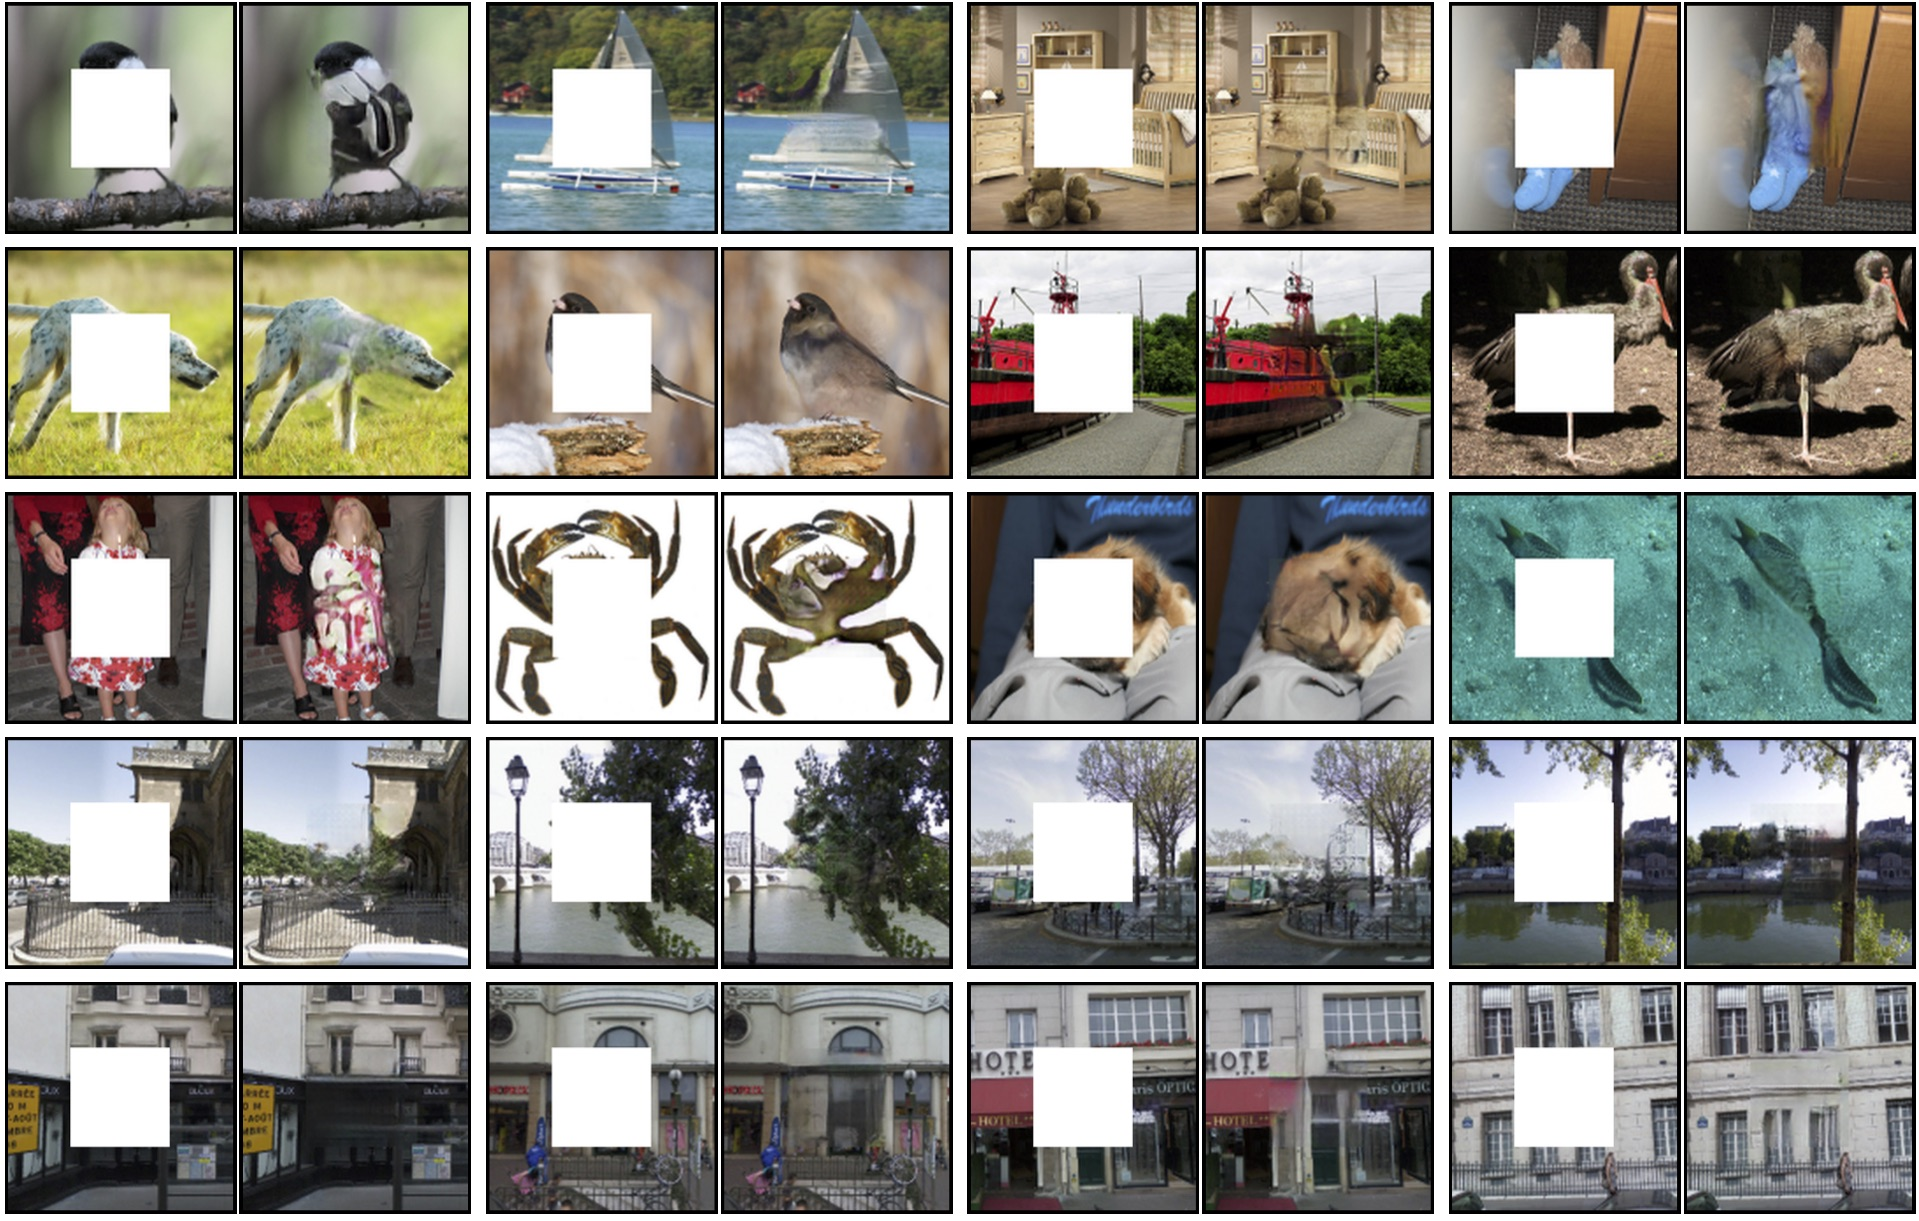
\includegraphics[scale=0.2]{teaser.jpg} 
                \caption{Exemples d'application}
            \end{figure}



    %%%%%%%%%%%%%%%%%%%%%%%
    %% TABLE DES FIGURES %%
    %%%%%%%%%%%%%%%%%%%%%%%
    \newpage
    \listoffigures
    \newpage



    %%%%%%%%%%%%%%%%%%
    %% BIBLIOGRAPHY %%
    %%%%%%%%%%%%%%%%%%
    \begin{thebibliography}{9}
        \bibitem{contextencoder} 
        Deepak Pathak, Phillip Krähenbühl, Jeff Donahue, Trevor Darrell, Alexei A. Efros
        \textit{Context Encoders: Feature Learning by Inpainting}. 
        UC Berkeley, CVPR, 2016.
        \\\texttt{https://people.eecs.berkeley.edu/\~{}pathak/context\_encoder}
    \end{thebibliography}


\end{document}

